\section{Durchführung}
\label{sec:Durchführung}

Der Vorteil eines Sagnac-Interferometers gegen\"uber anderen Interferometern ist die hohe Stabilit\"at der Strahlen, da diese durch den selben Strahlengang propagieren.
Im Folgenden wird zun\"achst auf den Aufbau und die Funktionsweise einen Sagnac-Interferometers eingegangen, bevor zum Schluss die Durchf\"uhrung und Messungen beschrieben werden.

\subsection{Aufbau}

In Abbildung \ref{fig:aufbau} ist der Versuchsaufbau dargestellt. Ein HeNe-Laser produziert monochromatisches Licht, welches \"uber die zwei Spiegel M1 und M2 auf einen
\textit{polarizing beam splitter cube} (PBSC) gelenkt wird. Ein PBSC teilt den eintretenden Strahl in zwei Strahlen auf die sich orthogonal zueinander ausbreiten und orthogonal zueinander
polarisiert sind. Die zwei Strahlen propagieren durch das eigentliche Interferometer, welches durch die Spiegel MA, MB und MC gebildet wird. Im Anschluss treffen die Strahlen erneut auf
den PBSC und werden Richtung Detektor weitergeleitet. Der Detektor besteht aus einem weiteren PBSC, der den Strahl teilt und auf zwei Photodioden lenkt, welche die Intensität messen.
Durch ein Polarisationsfilter im Strahlengang vor dem ersten PBSC, lässt sich der Anfangsstrahl beliebig linear polarisieren. Es ist möglich diverse Instrumente in den Strahlengang im Interferometer
zu stellen, um eine Phasendifferenz zwischen den Strahlen zu erzeugen.

\begin{figure}
  \centering
  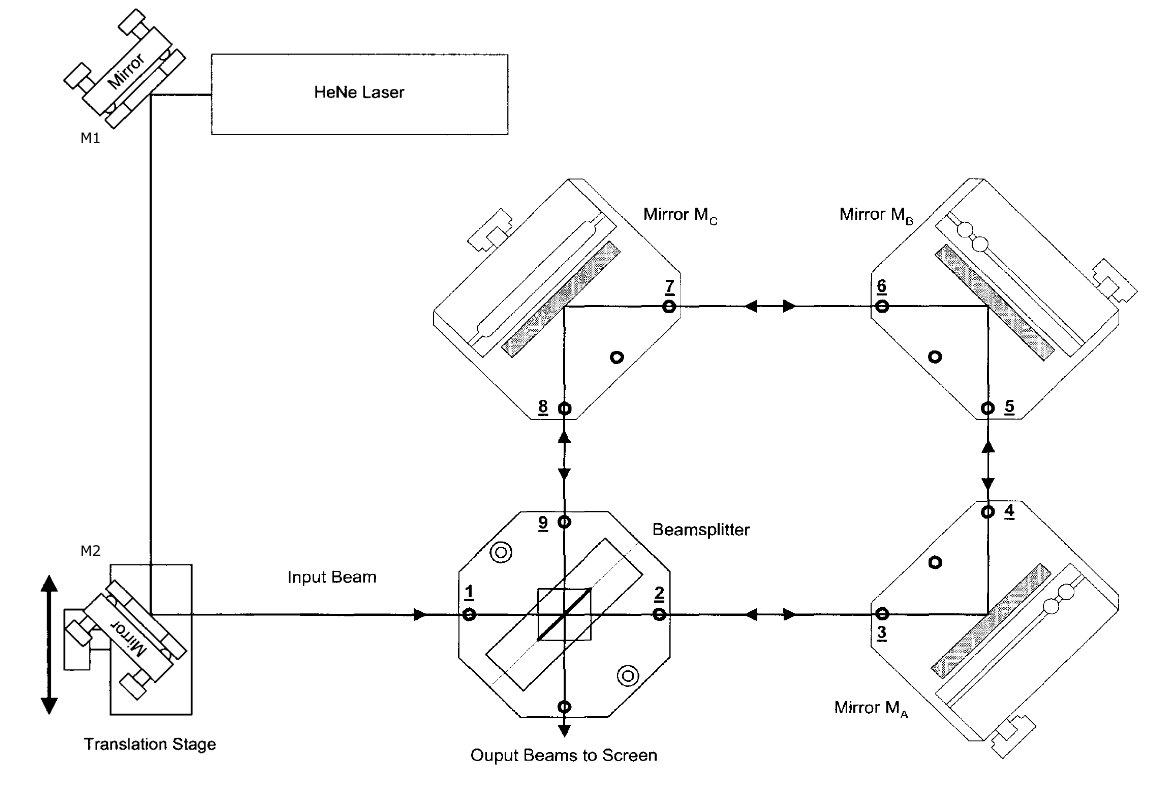
\includegraphics[width=0.7\textwidth]{aufbau.png}
  \caption{Eine Schematische Darstellung des Aufbaus \cite{anleitung}.}
  \label{fig:aufbau}
\end{figure}

\subsection{Justage}

Bevor Messungen zum Brechungsindex vorgenommen werden können, wird der Aufbau zunächst kalibriert. 
Dafür wird zuerst mittels Justageplatten, Feinjustierschrauben und Bodenplatten die passierenden Strahlen mittig auf die Spiegel M1, M2 und anschließend auf M3 gerichtet.
Dabei muss dringend bedacht werden, die Spiegel nach dem lösen der Schraube zum justieren wieder festzuschrauben.
Als Nächstes wird der Strahl nach dem erneuten Propagieren durch den PBSC betrachtet.
Da diese orthogonal zueinander polarisiert sind, sind keine Interferenzeffekte sichtbar.
Durch das einsetzen eines weiteren Polarisationsfilters mit einem Filterwinkel von 45° 
hinter dem PBSC, werden Interferenzeffekte sichtbar. Es gilt diese durch feinere Justage zu entfernen.

Um den Lichtstrahl in zwei parallele Strahlen zu teilen, wird der Spiegel M2 parallel zur
Oberfläche des PBSC bewegt. Es enstehen zwei Strahlen, die nach der zweiten
Propagation durch den PBSC auf einem Punkt fokusiert sind. 
Zus\"atzlich wird ein Rotationshalter in den Strahlengang innerhalb des Interferometers installiert. In diesem befinden sich zwei Glasplatten mit einer Dicke von $T=\SI{1}{\milli\metre}$.
Es steht jeweils ein Glas in dem Strahlengang von einem der Lichtstrahlen. Die beiden Glasplatten k\"onnen im Winkel zum Strahl bis zu 10° gedreht werden, wodurch ein Gangunterschied ensteht und
ein Interferenzmuster in Abh\"angigkeit vom Winkel der Glasplatten untersucht werden kann. 
Zum Schluss wird der zweite Polarisationsfilter
durch den zweiten um 45° gedrehten PBSC ersetzt, welcher die Strahlen auf beide Photodioden lenkt.

\subsection{Messung}

Als Erstes wird der Kontrast des Interferometers und dessen Abh\"angigkeit von der Polarisation gemessen. Daf\"ur wird
der Polarisationfilter in 15° Schritten gekippt und f\"ur jeden Filterwinkel das Maximum und Minimum der Intensit\"at mittels dem Rotationshalter untersucht und anschließend gemessen.
F\"ur die n\"achsten Messungen wird der Polarisationsfilter auf den h\"ochsten ermittelten Kontrast eingestellt.
W\"ahrend f\"ur die Messung des Kontrast die Intensität mit nur einer Photodiode gemessen wurde, wird in den folgenden Messungen stets die Differenzspannung der beiden Photodioden nach dem zweiten PBSC
verwendet. Der Vorteil liegt darin dass St\"oreffekte, wie Licht von \"au\ss{}eren Lampen, die sonst einen stetigen Offset erzeugen w\"urden zum gro\ss{}enteil verschwinden.

Als n\"achstes werden Messungen zur Bestimmung des Brechungsindex der Glasplatten durchgef\"uhrt. Daf\"ur wird zehnmal mit einem \textit{Modern Interferometry Controller} die Anzahl der Interferenzextrema
in Abh\"angigkeit vom Drehwinkel der Glasplatten gemessen.

Zuletzt wird f\"ur die Bestimmung des Brechungsindizes von Luft eine Gaszelle mit L\"ange $L=\SI{100.0(1)}{\milli\metre}$ in den Strahlengang eines Lichtstrahls eingebaut.
Die evakuuierte Gaszelle wird anschließend langsam mit Luft gef\"ullt, wobei die Anzahl der Interferenzextrema in Abh\"angigkeit vom Druck $p$ gemessen und alle $\SI{50}{\milli\bar}$ aufgezeichnet werden.
Diese Messung wird dreimal durchgef\"uhrt.